\documentclass{exam}

\usepackage{units} 
\usepackage{graphicx}
\usepackage[fleqn]{amsmath}
\usepackage{cancel}
\usepackage{float}
\usepackage{mdwlist}
\usepackage{booktabs}
\usepackage{cancel}
\usepackage{polynom}
\usepackage{caption}
\usepackage{fullpage}
\usepackage{xfrac}
\usepackage{enumerate}

\newcommand{\degree}{\ensuremath{^\circ}} 
\everymath{\displaystyle}

\printanswers

% \begin{figure}[H]
%   \centering
%   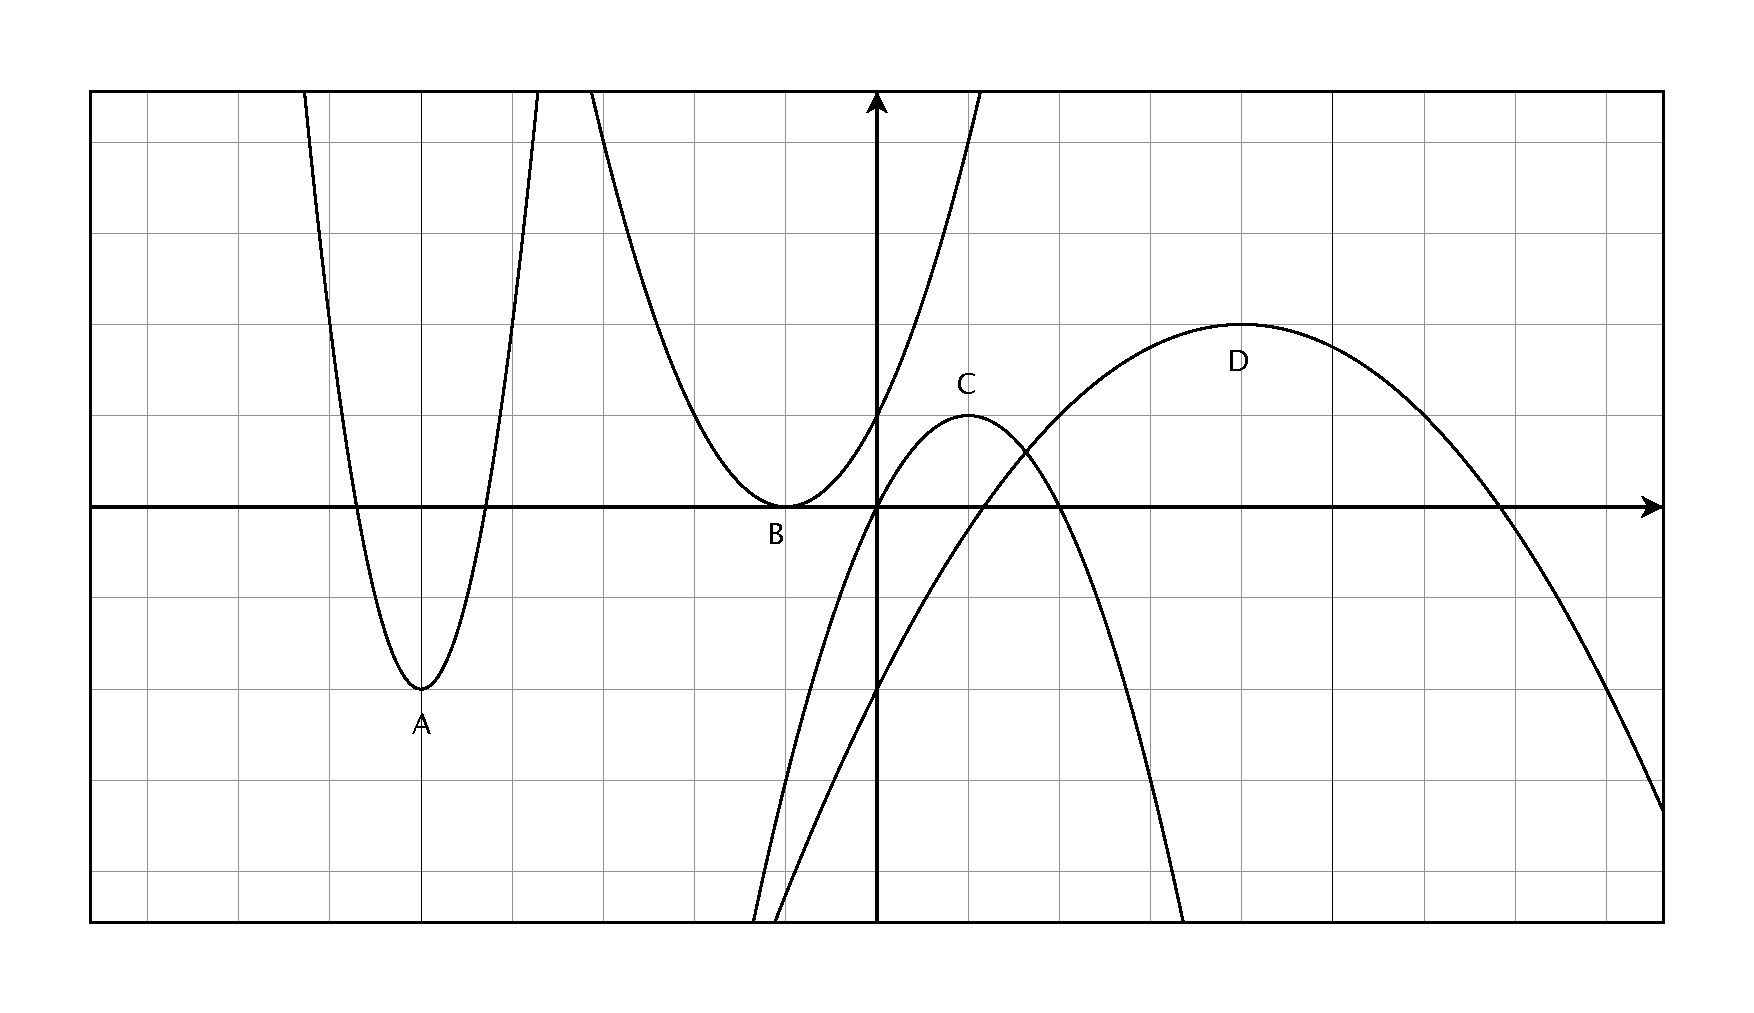
\includegraphics[scale=.3]{problem_7.eps}
%   \caption*{Problem 7}
% \end{figure}

% \begin{tabular}{cc}
% \toprule
% period & amplitude \\
% \midrule
%   $\pi$ & $2$ \\
% \bottomrule
% \end{tabular}

\title{Math 141 Notes \\ Section 4.2--Logarithms}

\date{June 12, 2013}

\begin{document}

  \maketitle
  \tableofcontents

  \section{History}
  \subsection{John Napier}

  \begin{itemize*}
    \item 1550-1617
    \item logarithms published 1614
    \item invented decimal point
    \item farmer
    \item invented submarine
    \item wrote popular book on religion predicting world would end between 1688 and 1700
    \item lie detecting chicken, drunken pigeons
  \end{itemize*}

  Idea: turn hard operations (multiply, divide, power) into easy operations (add, subtract, multiply) by working on
  exponents instead of numbers.

  Do table look up, calculation, reverse table look up

  examples 
  \begin{itemize*}
    \item $\sqrt[5]{17} \cdot \sqrt[4]{12}$
    \item $123456 \cdot 78912345$
  \end{itemize*}

  You don't need a table with every number since you can derive other numbers if you have a table from 0 to 10.  For
  example, if you know that 
  \[
    7 = 10^{0.8451}
  \]
  You can find:
  \[
    70 = 10 \cdot 10^{0.8451} = 10^{1.8451}
  \]

  Square root algorithm by repeated division.

  \begin{tabular}[H]{rr}
    \toprule
    $x$    & $10/guess$ \\
    \midrule
    3      & 3.3333 \\
    3.1667 & 3.1579 \\
    3.1623 & 3.1623 \\
    \bottomrule
  \end{tabular}

  \begin{tabular}[H]{rr}
    \toprule
    $x$    & $\sqrt{10}/guess$ \\
    \midrule
    1.5    & 2.1082 \\
    1.8041 & 1.7528 \\
    1.7785 & 1.7781 \\
    1.7783 & 1.7783 \\
    \bottomrule
  \end{tabular}

  Made table of fractional powers of 10 with repeated square roots.

  \begin{tabular}[H]{lr}
    \toprule
    $x$ & $10^x$ \\
    \midrule
    1/2 & 3.1623 \\
    1/4 & 1.7783 \\
    1/8 & 1.3335 \\
    1/16 & 1.1548 \\
    1/32 & 1.0746 \\
    1/64 & 1.0366 \\
    x & $1 + 2.3026x$ \\
    \bottomrule
  \end{tabular}

  \begin{align*}
    \log 7 &= 10^{1/2} \cdot 2.2136 \\
           &= 10^{1/2} \cdot 10^{1/4} \cdot 1.2448 \\
           &= 10^{1/2} \cdot 10^{1/4} \cdot 10^{1/16} \cdot 1.0779 \\
           &= 10^{1/2} \cdot 10^{1/4} \cdot 10^{1/16} \cdot 10^{1/32} \cdot 1.0031 \\
    \\
    1.0031 &= 1 + 2.2136x \\
    0.0031  &= 0.2136x \\
    x      &= 0.0014
    \\
    \log 7 &= 10^{1/2} \cdot 10^{1/4} \cdot 10^{1/16} \cdot 10^{1/32} \cdot 10^{0.0014} \\
           &= 10^0.8452 \\
  \end{align*}

  Show another example of calculation.

  \subsection{After Napier}

  \begin{itemize}
    \item Briggs (1561-1631) changed details of calculation to match current base 10 logarithms.  From 1614-1624
      calculated all integers from 1-20,000 and 90,000 to 100,000.  

    \item Adrian Vlacq (1600-1667) filled in gaps for second edition in 1628.

    \item From 1924-1949 new set of tables calculated.

    \item Computers used after around 1950.
  \end{itemize}

  \pagebreak

  \section{Definitions}

  \[
    \log_{10} x = a \Longleftrightarrow 10^a = x
  \]

  examples:
  \begin{align*}
    \log_{10} 100 &= 2 \\
    \log_{10} 1 &= 1 \\
    \log_{10} \frac{1}{10} &= -1 \\
  \end{align*}

  General
  \[
    \log_b x = a \Longleftrightarrow b^a = x
  \]

  examples:
  \begin{align*}
    \log_6 36 = 2 & \Longleftrightarrow 6^2 = 36 \\
    \log_2 32 = 5 & \Longleftrightarrow 2^5 = 32 \\
    3^4 = 81 & \Longleftrightarrow \log_3 81 = 4 \\
    2^{-3} = \frac{1}{8} & \Longleftrightarrow \log_2 \frac{1}{8} = -3 \\
    10^3 = 1000 & \Longleftrightarrow \log_{10} 1000 = 3 \\
  \end{align*}

  more examples:
  \begin{align*}
    \log_5 5^4 &= 4 \\
    \log_7 \left( \frac{1}{49} \right) &= -2 \\
    \log_{11} 11 &= 11 \\
    \log_4 2 &= \log_4 4^{1/2} = \frac{1}{2} \\
    \log_{25} \sqrt{5} = \log_{25} \left( 25^{1/2} \right)^{1/2} \\
  \end{align*}

  \section{Equations With Logarithms}
  \begin{align*}
    \log_2 x &= 5 \\
    x        &= 32 \\
  \end{align*}
  
  \begin{align*}
    \log_7 x &= \frac{1}{2} \\
    x        &= \sqrt{7} \\
  \end{align*}

  \begin{align*}
    \log_x 36 = 2 \\
    36               &= x^2 \\
    x                &= 6 \\
  \end{align*}

  \begin{align*}
    \log_x \left( \frac{1}{10} \right) &= -1 \\
    \frac{1}{10}                       &= x^{-1} \\
    x                                  &= 10 \\
  \end{align*}

  \section{Graphs}

  \begin{figure}[H]
    \centering
    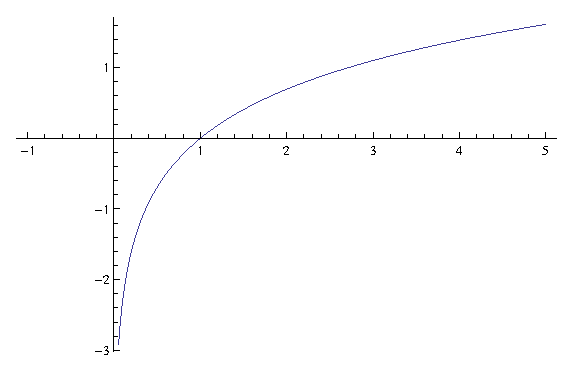
\includegraphics{figure1.eps}[scale = 1.0]
    \caption{$\log_2 x$}
  \end{figure}

  Move graph around
  \begin{itemize*}
    \item $\log_2 (x - 3)$
    \item $(\log_2 x) - 3$
    \item $- \log_2 x$
    \item $\log_2 (-x)$
  \end{itemize*}
  
  \pagebreak

  \section{Carbon 14 Dating}

  Half life of Carbon 14 is 5,730 years.

  Like compound interest running time in reverse. Principal is amount present today and amount is the amount present in
  the past.

  \begin{align*}
    A      &= P e^{rt} \\
    \\
    D_0    &= D e^{rt} \\
    e^{rt} &= \frac{D_0}{D} \\
    rt     &= \ln{\frac{D_0}{D}} \\
    \\
    r \cdot 5730 &= \ln{2} \\
    r            &= \frac{\ln{2}}{5730} \\
                 &= 0.000120968 \\
    \\
    t &= \frac{1}{r} \cdot \ln{\frac{D_0}{D}} \\
      &= 8267 \ln{\frac{D_0}{D}} \\
  \end{align*}

  When 60 grams out of 100 are left:
  \[
    t = 8267 \ln{\frac{100}{60}} = \unit[4223]{years}
  \]

\end{document}
